
\subsection{Design and methodology}
This section of the document is dedicated to the explanation of how user testing has been designed and then put in practice for the \href{https://www.unicef.org/}{UNICEF website}.
As mentioned in the introductory part (\hyperref[subsec:introUT]{section 2.1}), the first phase is the setup of the entire user testing procedure.\\
First off, the user profile that has been chosen for this test can be defined as a person (male or female) in their twenties (so in a age range between twenty and thirty years old) who is interested in some of the topics and areas covered by the \href{https://www.unicef.org/}{UNICEF website}. The reasons why this choice was made are a few. To start with, people in this age range are expected to be rather skilled in using technological devices like laptops and also in searching information on the internet. This way, the tests are not undermined by lack of knowledge in these fields, which might happen with a higher probability in case of older people over thirty years old. Moreover, people between twenty and thirty years old are more likely to have a ground knowledge on at least some of the areas UNICEF is involved in, because of social media and the constant circulation of information around those important topics for the modern society.\\
The number of users per inspector to be recruited has been set to 5, following Nielsen's rule, which states that with 5 users it is possible to catch 85\% of usability problems on the website under analysis.\\
As for the quantitative and qualitative variables to be measured during the tests, the following is an image representing the form used by all inspectors to annotate the users' performances and behaviours:

\begin{center}
	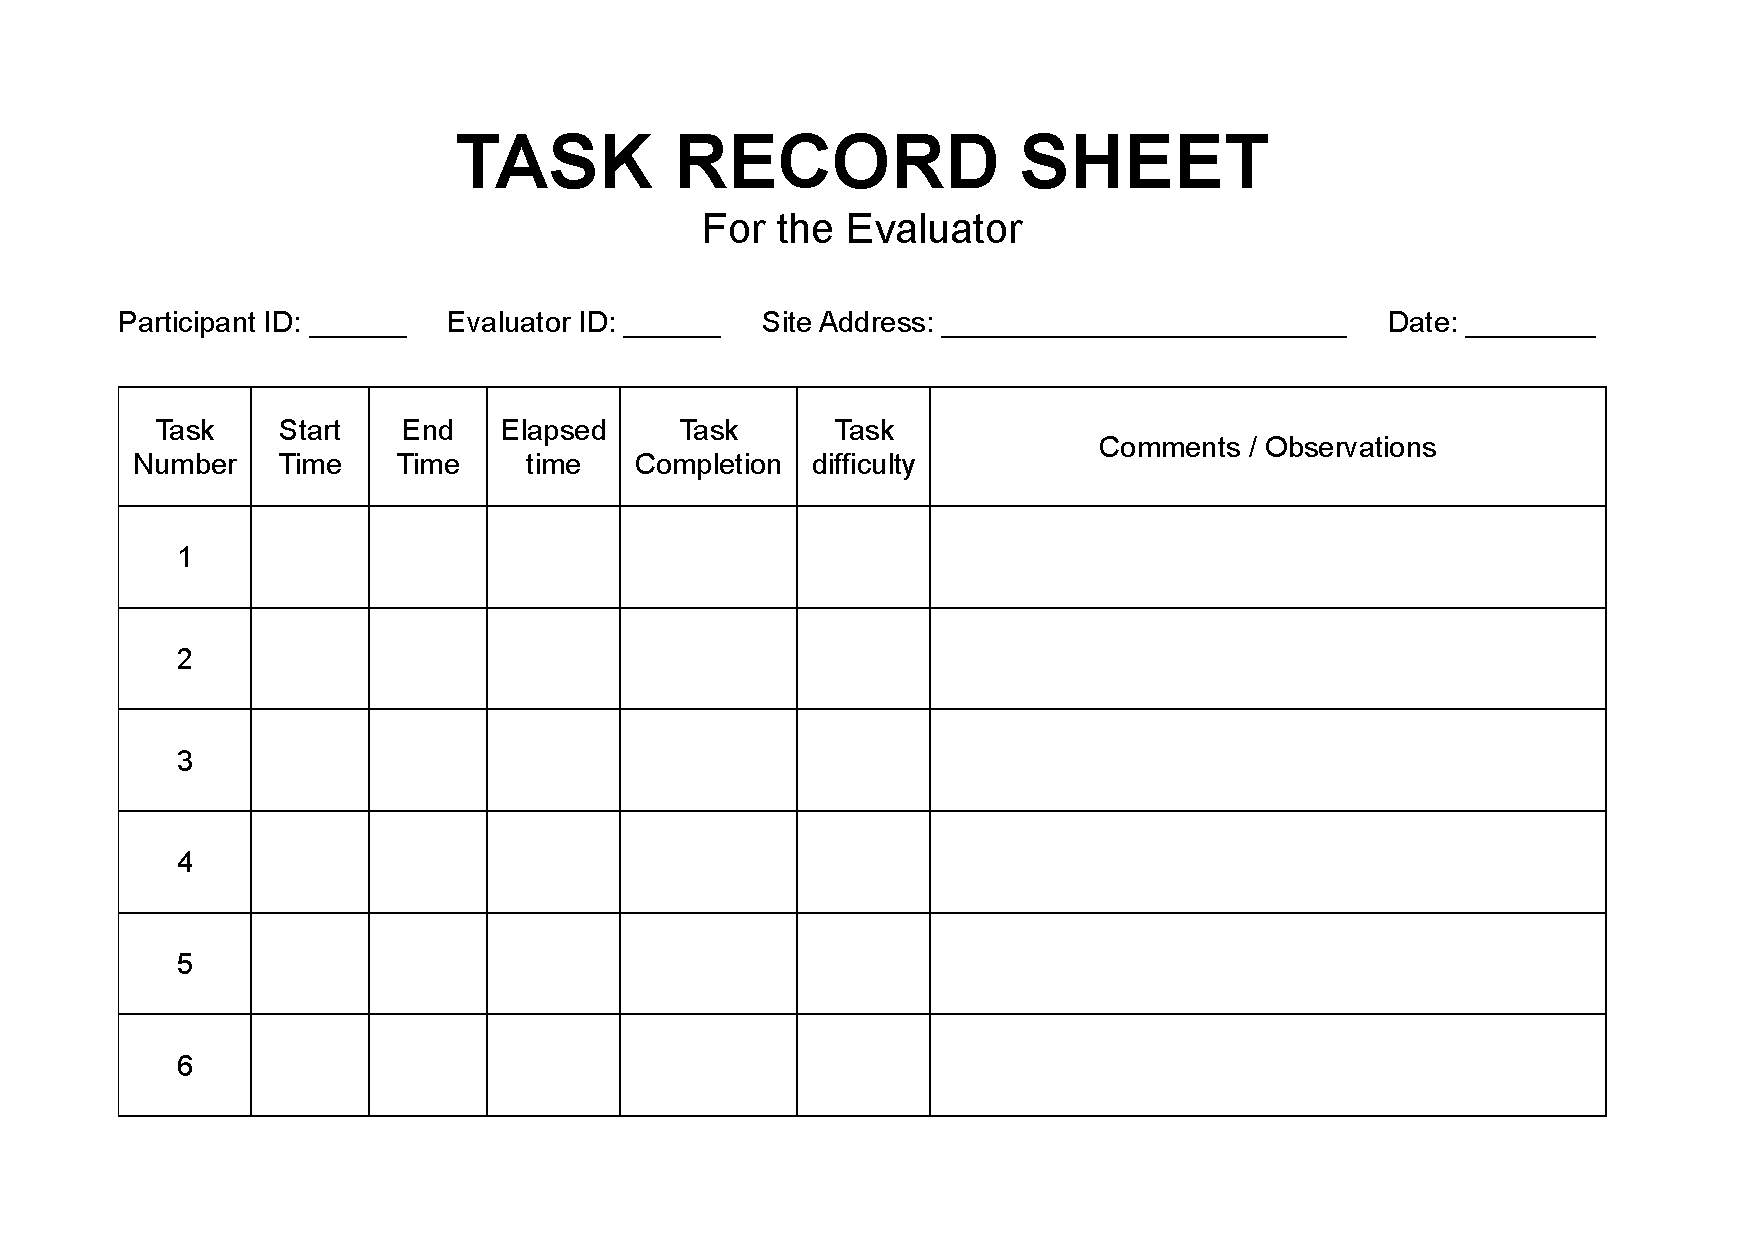
\includegraphics[width=0.8\textwidth,page=1]{\utRes/CollectionData.pdf}
\end{center}

\clearpage
It is possible to notice the following metrics that are extracted from the experts during the tests:
\begin{itemize}
	\item \textbf{Start Time}: exact time in which the user starts reading the text for the corresponding task, with a granularity of seconds.
	\item \textbf{End Time}: exact time in which the user finishes the task, either by giving up (failing) or by providing the inspector with the correct answer. Again, this variable is given with the granularity of seconds.
	\item \textbf{Elapsed Time}: time passed between the Start Time and the End Time, with granularity of seconds.
	\item \textbf{Task Completion}: this metric has been defined with the following possible values and corresponding meanings:
		\begin{enumerate}
			\item \textbf{Failure}: the user is unable to find the solution and s/he gives up without even getting close to the result. Not even an hint helps the user accomplish the task.
			\item \textbf{Partial}: the user finds a partial solution, meaning that s/he manages to reach the correct section of the website and understands how the navigation should be performed, but s/he struggles with providing a definitive answer to the task.
			\item \textbf{Completed ASSISTED}: the user completes the task, but only after receiving a little hint from the inspector on how to find a way to the solution.
			\item \textbf{Completed ALT}: the user completes the task, but in an ALTernative way compared to the "standard" one expected and designed by the evaluators at task creation time. The expected navigation paths can be found in the task sheets in the following of this chapter.
			\item \textbf{Completed}: the user completes the task after a few attempts, without needing any input from the inspector and in the "standard" way compliant to the design of the task.
		\end{enumerate}
	\item \textbf{Task Difficulty}: estimates the level of cognitive effort requested by the user to complete the task, with a value ranging from 1 to 5 based on the observed level of ease of use or struggling in finding the solution. \\ Regarding the range of values for this metric, the value 1 was given in case the user was clearly confident from the very beginning on the navigation path to reach the target. The perceived difficulty incrementally increases as the value assigned gets closer to 5. The value of 5 is given only when the user shows frustration multiple times and the completion of the task requires a lot of time (or the task is not even completed).
\end{itemize}

Finally, in the \textit{Task Record Sheet} a \textbf{Comments/Observations} section is included to annotate all the actions taken and reactions observed from the user while interacting with the website.
As an additional source of information that seemed to be relevant in the design phase of this process, a \textit{Post-test Questionnaire} was also created to gather other important ideas or thoughts that the user had while performing the tasks. Most of the variables defined in this questionnaire are qualitative, as they are based on the perception and feelings that the user had during the process.
Here's a copy of the questionnaire for the reader:

\begin{center}
	\includegraphics[width=0.8\textwidth,page=2]{\utRes/CollectionData.pdf}
	\includegraphics[width=0.8\textwidth,page=3]{\utRes/CollectionData.pdf}
\end{center}

The results of the \textit{Task Record Sheets} and the \textit{Post-test questionnaire} for each user involved in the tests can be found in the \hyperref[sec:annex]{Annex section} of this document.\\
The metrics and measures inserted in these sheets have to be considered as the raw data set elicited from the users at testing time. In the section \hyperref[subsec:resultsUT]{Usability indicators and final scores}, this raw data set is processed and many other indicators and metrics are elicited from it.
 
 
 
Moving on to the design of the tasks, the reader is provided with a copy of the \textit{Task Sheet} that was delivered to all the users recruited for the test. The following three pages accommodate this \textit{Task Sheet}. It is relevant to notice that the last page of this sub-document is dedicated to the descriptions of the task solutions. More specifically, it is possible to find here the navigation paths inside the \href{https://www.unicef.org/}{UNICEF website} that the evaluators identified as the "standard" ones to reach the solutions of the various tasks (so the most straightforward or expectable ones). These paths have been determined based on an accurate inspection of the \href{https://www.unicef.org/}{UNICEF website} (described in \hyperref[sec:inspection]{Section 1} of this document). 

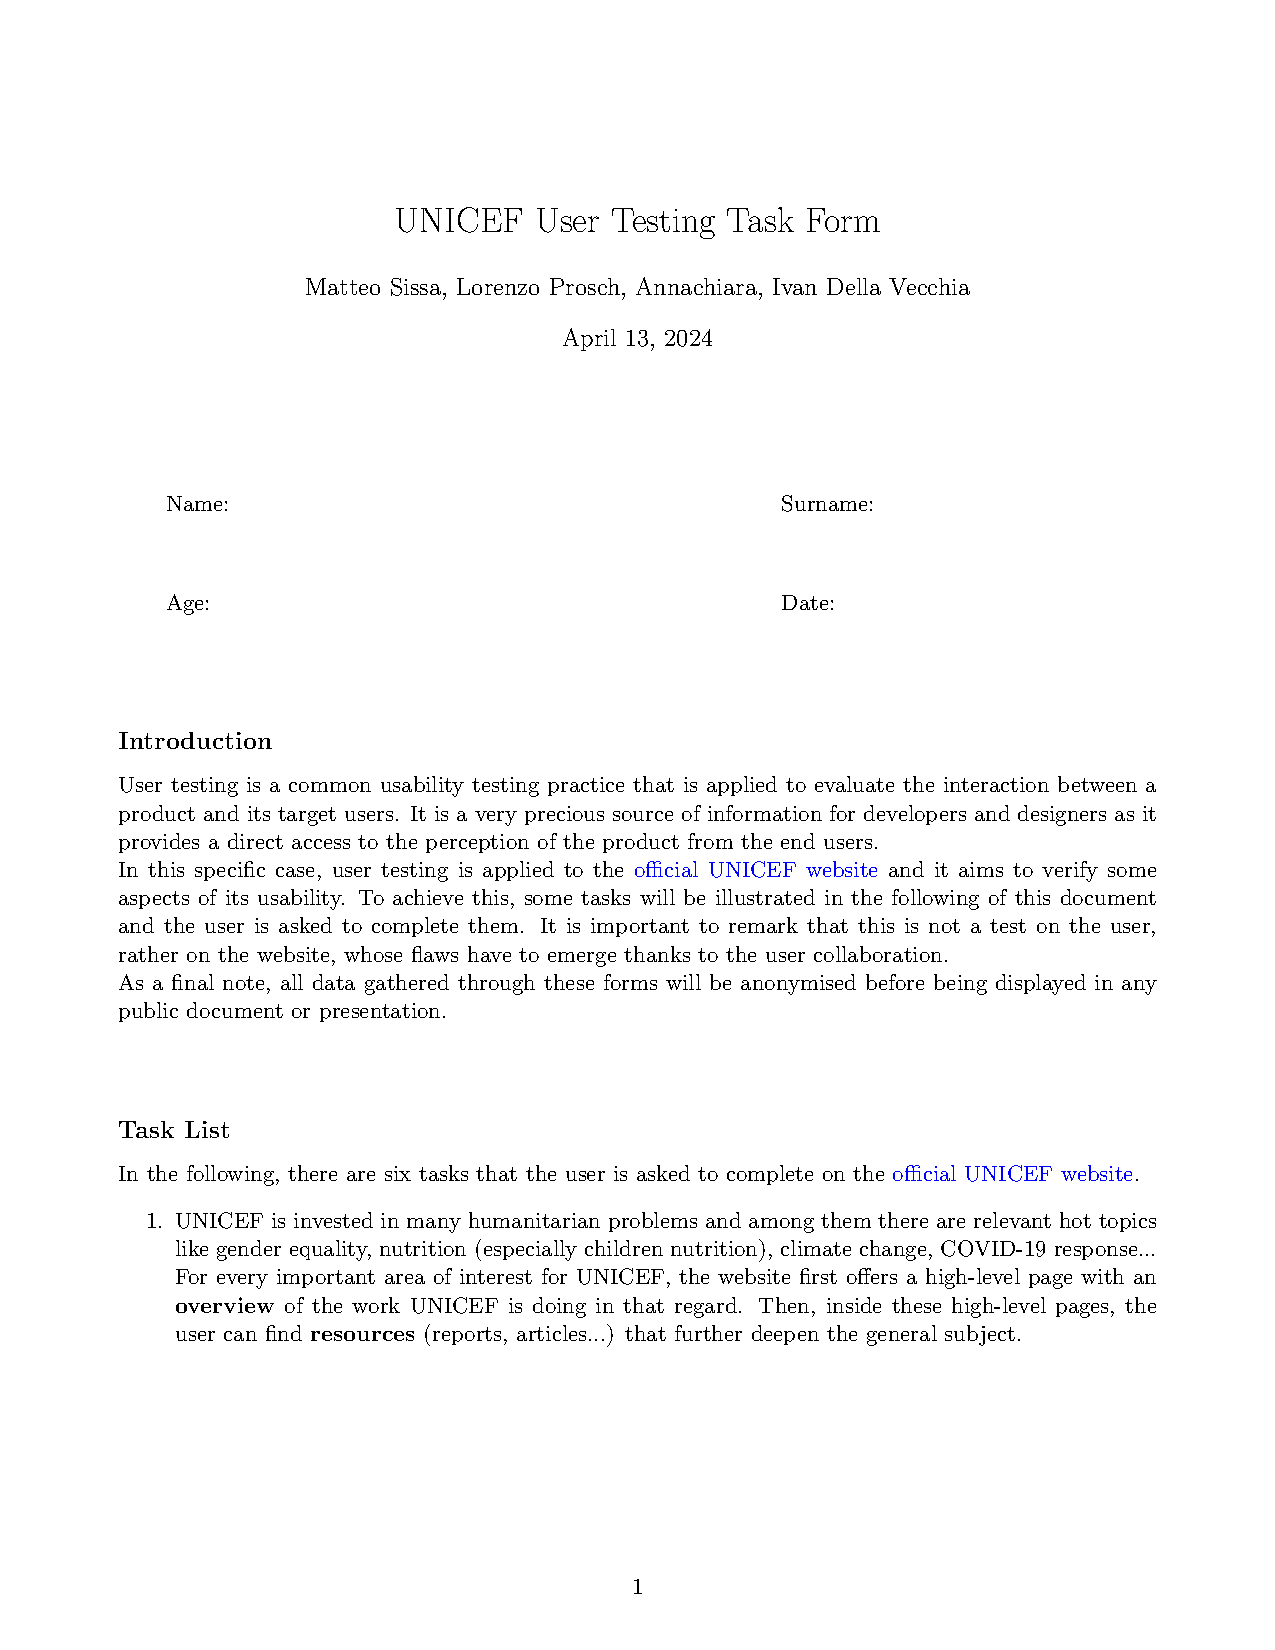
\includepdf[pages=-]{\utRes/TaskForm.pdf}
	
Some remarks are needed, to let the reader better understand how the tasks have been designed and fabricated. 
The total time of execution of the tasks has been estimated around 35 minutes, also counting in the time required to fill out the post-test questionnaire. More specifically, the following timings are the ones expected for the completion of the tasks, also based on their complexity for an inexperienced user:

\vspace{0.5cm}

{
	\renewcommand{\arraystretch}{1.45}
	\setlength{\tabcolsep}{0.5cm}
	\centering 
\begin{tabular}{c| c c c c c c}
	Task n° &1 & 2 & 3 & 4 & 5 & 6\\
	\hline
	Time & 6min & 4min & 3min & 6min & 3min & 3min
	
\end{tabular}

}

\vspace{0.5cm}

Furthermore, all the tasks have been tailored specifically around the results of the inspection procedure, described in the first chapter of this document. The inspection has shed a light on many issues that the \href{https://www.unicef.org/}{UNICEF website} presents, so the purpose of the tasks is also to validate this analysis by "forcing" the users to navigate to specific sections of the website where the problems have emerged. Thanks to this approach, the behaviour of the users can confirm or disproof some of the points that have been elicited from the inspection.\\
The tasks have also been designed to be suitable for users interested in what UNICEF has to offer. They represent common jobs that any person on the website should be able to carry out with little effort. Obviously, the user profile described earlier has also been accounted for when writing the tasks down.\\
As a final note, the task sheet attached to this document has been subject to some adjustments and changes deriving from a couple of pilot tests organised with additional users whose results aren't included in the analyses of this document. Thanks to these pilot tests, some ambiguities in the way tasks were presented emerged and they were successfully resolved before starting with the "real" tests.\\

The last part about methodology to be addressed regards the actual \textbf{execution} of the study, so the setting and environment that was established among evaluators to make the analyses uniform over all users.
In this case, all inspectors agreed on making the user perform the tasks on a laptop or a computer, and avoid any other type of device (e.g. tablet, mobile phone, IoT devices...). Moreover the environment chosen for the execution of the tests had to be silent and possibly isolated from any external distraction (other people around, television, external noise...).
As a support for analysis, it has also been established to record the user's voice during the test in order to be able to listen again to comments and impressions on the website if necessary.

In the following of this document, the results of the user testing procedure on the \href{https://www.unicef.org/}{UNICEF website} are illustrated, also by means of visual and graphical representations to help the reader understand the findings of this research.
	

